\documentclass[journal]{IEEEtran} % use the `journal` option for ITherm conference style
\IEEEoverridecommandlockouts
% The preceding line is only needed to identify funding in the first footnote. If that is unneeded, please comment it out.
\usepackage{cite}
\usepackage{amsmath,amssymb,amsfonts}
\usepackage{algorithmic}
\usepackage{graphicx}
\usepackage{textcomp}
\usepackage{xcolor}
\usepackage{hyperref}
\def\BibTeX{{\rm B\kern-.05em{\sc i\kern-.025em b}\kern-.08em
    T\kern-.1667em\lower.7ex\hbox{E}\kern-.125emX}}
\begin{document}

\title{Using Ethereum Blockchain for distributed marketplace\\
% delete or comment-out the following line before submission
%{\footnotesize \textsuperscript{*}Note: Sub-titles are not captured in Xplore and should not be used}
%\thanks{Identify applicable funding agency here. If none, delete this.}
}

\author{%%%% author names
    \IEEEauthorblockN{1\textsuperscript{st} Naveen Kumar Muga}% first author
    , \IEEEauthorblockN{2\textsuperscript{nd} Pardhavi Reddy Jonnala}% delete this line if not needed
    , \IEEEauthorblockN{3\textsuperscript{rd} Shana T. Haynes}% delete this line if not needed
    % duplicate the line above as many times as needed to list all authors
    \\%%%% author affiliations
    \IEEEauthorblockA{\textit{UAB, Alabama, US}}\\% first affiliation
    %\IEEEauthorblockA{\textit{dept. name of organization (of Aff.), City, Country if needed}}\\% delete this line if not needed
    % duplicate the line above as many times as needed to list all affiliations
    %%%% corresponding author contact details
    %\IEEEauthorblockA{email address or ORCID of corresponding author(s)}
}

\maketitle

\begin{abstract}
    This document is a attempt to research possibility of creating Dark Web markets on Ethereum blockchain in fully distributed manner.
\end{abstract}

\begin{IEEEkeywords}
    React.js, blockchain, ethereum, DarkWeb, market
\end{IEEEkeywords}

\section{Introduction}
This document is a model and instructions for minimal distributed marketplace setup and technology stack description for extending it further.

\section{Background}

    \subsection{Brief History}
    Darknet markets — also known as cryptomarkets — provide a largely anonymous platform for trading in a range of illicit goods and services. Most of them are drugs, freud related guides, 0-day exploits, hacked datasets with personal information and stolen credit cards data (CC's). Their around the internet from year 2010 and most of them is enduring for about 4 years. Giving their owners significant income. They operate as hidden service on anonymous network called Tor.

    \subsection{Tor network}
    Tor, short for The Onion Router, is free and open-source software for enabling anonymous communication. It directs Internet traffic through a free, worldwide, volunteer overlay network, consisting of more than seven thousand relays, to conceal a user's location and usage from anyone performing network surveillance or traffic analysis. Using Tor makes it more difficult to trace a user's Internet activity. Tor's intended use is to protect the personal privacy of its users, as well as their freedom and ability to communicate confidentially through IP address anonymity using Tor exit nodes.\\

    \subsection{Hidden service}
    A hidden service is a site or a service that uses Tor technology to stay secure and, if the owner wishes, anonymous. This services are internal to Tor network and offer bi-directional security by means of anonymity hiding server and client IP address from each other.\\

    \subsection{Blockchain}
    A blockchain is a type of distributed ledger technology (DLT) that consists of growing list of records, called blocks, that are securely linked together using cryptography. Each block contains a cryptographic hash of the previous block, a timestamp, and transaction data. The timestamp proves that the transaction data existed when the block was created. Since each block contains information about the previous block, they effectively form a chain (like linked list data structure), with each additional block linking to the ones before it. Consequently, blockchain transactions are irreversible in that, once they are recorded, the data in any given block cannot be altered retroactively without altering all subsequent blocks.\\

    \subsection{Smart Contracts}
    A smart contract is a transaction protocol that is intended to automatically execute, control or document events and actions according to the terms of a contract or an agreement. The objectives of smart contracts are the reduction of need for trusted intermediators, arbitration costs, and fraud losses, as well as the reduction of malicious and accidental exceptions. Smart contracts are commonly associated with cryptocurrencies, and the smart contracts introduced by Ethereum are generally considered a fundamental building block for decentralized finance.\\

\section{Description}
This program is a web based application implementing very basic advertisement website that allows exchange goods and services for cryptocurrency based on Ethereum blockchain utilizing SmartContracts. All of application data is stored in decentralized way whether it's an advertisement or transaction history. This is done by using two decentralized technologies first previously mentioned blockchain as ledger and the second Inter Planetary Filesystem for storing advertisements. Site enables users that owns Ethereum wallet address to post advertisement and the others to buy a service or good anonymously. What is main difference from previously known DarkWeb markets that no data other than application code is stored on one central server.

    \subsection{Ethereum}
        Ethereum allows anyone to deploy permanent and immutable decentralized applications onto it, with which users can interact. Decentralized finance (DeFi) applications provide a broad array of financial services without the need for typical financial intermediaries like brokerages, exchanges, or banks, such as allowing cryptocurrency users to borrow against their holdings or lend them out for interest. Ethereum also allows users to create and exchange NFTs, which are unique tokens representing ownership of an associated asset or privilege, as recognized by any number of institutions. Ethereum provides following sub components that allows application building:\\
            \subsubsection{Ethereum Virtual Machine (EVM)}
                The Ethereum protocol itself exists solely for the purpose of keeping the continuous, uninterrupted, and immutable operation of this special state machine. It's the environment in which all Ethereum accounts and smart contracts live. At any given block in the chain, Ethereum has one and only one 'canonical' state, and the EVM is what defines the rules for computing a new valid state from block to block.\\
                
            \subsubsection{Solidity}
                Solidity is an object-oriented, high-level language for implementing smart contracts. Smart contracts are programs which govern the behaviour of accounts within the Ethereum state. Solidity is a curly-bracket language designed to target the Ethereum Virtual Machine (EVM). It is influenced by C++, Python and JavaScript.\\
            
    \subsection{Interplanetary File System (IPFS)}
        The Interplanetary File System (IPFS) is a decentralized file system for building the next generation of the internet. Filecoin and many popular Web3 projects are built on IPFS. Some call it the hard drive for blockchain and Web3, though its power extends much further. This distributed hash based filesystem enables developers to store data like images or product description in decentralized manner. 

\section{Design}
    \subsection{Libraries}
        The following libraries were used to build application:\\
        
        \begin{description}
        
            \item[React] a free and open-source front-end JavaScript library for building user interfaces based on UI components. It is maintained by Meta (formerly Facebook) and a community of individual developers and companies. React can be used as a base in the development of single-page, mobile, or server-rendered applications\\
        
            \item[Web3] a collection of JS libraries that lets you interact with an Ethereum node remotely or locally. Simply, it provides us with an API to use so we can easily work with the blockchain. Web3 works as a wrapper for JSON RPC to connect to a remote or local Ethereum node with either a HTTP or IPC connection.\\
            
            \item[js-ipfs] a full P2P protocol written entirely in JavaScript it paves the way for the browser implementation of the IPFS protocol. Allowing to access decentralized storage directly from web browser.\\
            
        \end{description}
        
    \subsection{Architecture}
        Application consists of three layers:\\
    
        \subsubsection{Application}
            This part of application runs in user (seller, buyer) web browser with direct access to decentralized storage and ledger that is provided by Web3 and js-ipfs libraries. Actions like posting sell offer or buying service or goods are realized in end user web browser. Middleware HTTP server is only used to distribute application among users. While the IPFS access is truly direct, access to distributed ledger is done via so called HTTP RPC gateway multiple of such RPC nodes with public address is managed by community.\\
            
        \subsubsection{Middleware}
            That can be broke into two component one which is HTTP server based backend responsible for rendering the Application. When user connects to HTTP server his rendered page is downloaded by a browser together with set of libraries allowing access to decentralized ledger and storage.\\
        
        \subsubsection{Distributed Ledger}
            Distributed ledger is used for storing transactions and advertisement state, it is also used for executing state change when some of the actions happen. This actions are posting advertisement and buying. 
    
        The conceptual architecture is presented on Fig. \ref{fig}.
        
        \begin{figure}[htbp]
            \centerline{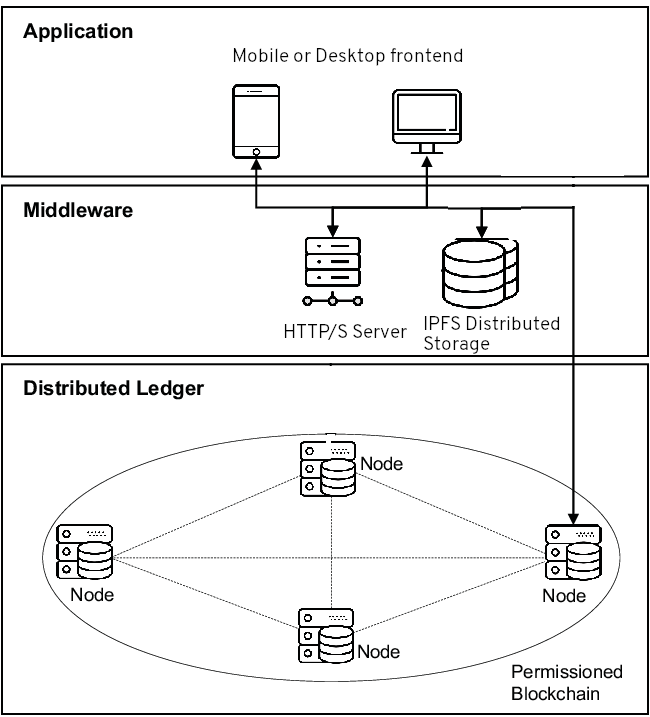
\includegraphics{arch.png}}
            \caption{Design schema}
            \label{fig}
        \end{figure}
    
    
    
\section{Design Decisions}
    \subsection{Common Pitfalls of Previous Markets}
        \subsubsection{Storing blockchain}
            Most of the previous DarkWeb markets used to run Bitcoin(BTC) or Monero(XMR) daemon on same host with application and http server for fast transaction processing and avoiding timeouts. Major pitfall of this approach is storing arbitrary large data as ~400GB for BTC and ~100GB for XMR.\\
            
        \subsubsection{Storing products}
            Storing products data such as description or images also requires large amount of storage while the number of products increases. It also produces one more requirement for CPU and RAM for searching and indexing this data. While traditionally data like images resides on hard drive for indexing DBMS (SQL,NoSQL) were used. No matter of used DBMS technology additional computing power was required. Commonly for accelerating search of products other technologies were involved such Redis or Elasticsearch.\\
            
        \subsubsection{Serving application}
            Web applications made in scripting languages geared towards web development required even more computing power when traffic on such sites become larger. Later versions of Tor router provided a way for High Availability of HTTP server and scripting backend behind them.\\
            
        \subsubsection{Handling large traffic}
            While the number of users was increasing on such markets the traffic volume was also increasing because of need to serve product mostly product data such as images to buyers and vendors. Traffic analysis performed by government authorities was a way for seizing some of the this criminal sites.\\
            
        Previously mentioned pitfalls caused such market sites to be very complex in design and vulnerable to exploiting by finding configuration mistakes or DDoS attacks. New decentralized approach gets rid of them.
        
    \subsection{New approach}
        \subsubsection{Storing blockchain}
            Using decentralized approach allows end users to connect directly to various hosts serving HTTP RPC service for accessing Ethereum blockchain eliminating single point of failure and making traffic distributed among internet hosts. With no need of storing arbitrary large blockchain data.\\
            
        
        \subsubsection{Storing products}
            Decomposing traditional DBMS system into two components blockchain and object storage (IPFS) allows of storing even large dataset without a need of extra disk space and removes the need for additional tools such as caching or searching accelerators like Redis or Elasticsearch. The blockchain in this approach is used as index for object storage lying on IPFS.\\
            
        \subsubsection{Serving application}
            While using blockchain and decentralized storage there is no need for additional computing power on a server that is distributing application to end users, because the only dynamic element that might change in time are addresses of remote Ethereum blokchain RPC nodes. That can be fetched by web browser application from additional service. Thanks to that application can be cached by the web server and served as static page.\\
        
        \subsubsection{Handling large traffic}
            Without serving images data by application HTTP server traffic volume even with large number of users and requests drops significantly as only text data is distributed to users. All of the other data is fetched by their browsers from decentralized storage.
            
    \subsection{Proof of Concept}
        PoC was build using React.js because makes it quick and painless to create interactive UIs. Application is build of simple product view with ability to post new product listing by vendor and buy it by consumer. All of the view changes happen just in a web browser without further requests to HTTP server distributing application.

\section{Limitations}
    With a limited time for preparing PoC many important features are missing in it to be competitive with other DarkWeb markets. There is no:
    \begin{enumerate}
        \item Messaging system
        \item Escrow system
        \item Vendor reputation system
        \item Product comments
    \end{enumerate}
    
    \subsection{Future Work}
        \subsubsection{Messaging system}
            While on previous DarkWeb markets BitMessage, or some internal implementation of messaging storing messages in DBMS was used here IPFS object storage can be used to store messages between users as of privacy concern this messages should be like in previous solutions encrypted using for example very popular among Tor network PGP public/private key system.\\
            
        \subsubsection{Escrow - buyer/seller protection}
            While the objectives of smart contracts are the reduction of need for trusted intermediators, arbitration costs, and fraud losses, as well as the reduction of malicious and accidental exceptions. There is no possibility of buyer protection when only parties of transaction are buyer and seller. There must be trusted third party involved between buyer and seller. When transaction is between two of them and seller won't send the physical or digital product buyer can complain to seller only and only his good will can toward to resolve the problem. When there're is a trusted third party introduced and seller doesn't gets his money when transaction is done by buyer, but funds are transferred into newly created account which is owned by buyer, seller and third party and to make a withdrawal there must be 2 of 3 consensus seller has the motivation to resolve issue. This is how multisignature addresses or wallets work in fg. Bitcoin network. In case of conflict between buyer and seller they can contact this trusted third party for arbitration and this person sign buyers withdrawal or buyers refund on blockchain allowing one of them to get funds. If there is no conflict between them seller can sign withdrawal and buyer can confirm it without contacting arbitrator. Such an example implementation exists \href{https://solidity-by-example.org/app/multi-sig-wallet/}{here}\\
            
        \subsubsection{Vendor reputation system}
            Vendor reputation system can be easily implemented after adding multisignature wallets as ratio between transactions from which seller withdraw funds to overall transactions.\\
            
        \subsubsection{Product comments}
            Comments and any additional product data can be implemented suing IPFS object storage and using blockchain as index\\
            
        Blockchain technologies involved in this project gives one more opportunity for developers of similar applications that are auto shops. As after every transaction and payment made by buyer event can be emitted and catched digital products such as stolen credit cards data with personal data can be auto delivered to buyer. Making personality thefts even more easier. 
         
\section{Conclusion}
    While blockchain and decentralization are beneficial to many branches of economy and industry they also bring new potential threats that can be used by cyber criminals to continue their activity and avoid arresting. While this new technologies emerge government authorities and law enforcement should prepare new investigation techniques of beating it.
%\section*{References}

%Please number citations consecutively within brackets \cite{b1}. The
%sentence punctuation follows the bracket \cite{b2}. Refer simply to the reference
%number, as in \cite{b3}---do not use ``Ref. \cite{b3}'' or ``reference \cite{b3}'' except at
%the beginning of a sentence: ``Reference \cite{b3} was the first $\ldots$''

%Number footnotes separately in superscripts. Place the actual footnote at
%the bottom of the column in which it was cited. Do not put footnotes in the
%abstract or reference list. Use letters for table footnotes.

%Unless there are six authors or more give all authors' names; do not use
%``et al.''. Papers that have not been published, even if they have been
%submitted for publication, should be cited as ``unpublished'' \cite{b4}. Papers
%that have been accepted for publication should be cited as ``in press'' \cite{b5}.
%Capitalize only the first word in a paper title, except for proper nouns and
%element symbols.

%For papers published in translation journals, please give the English
%citation first, followed by the original foreign-language citation \cite{b6}.

%\begin{thebibliography}{00}
%    \bibitem{b1} G. Eason, B. Noble, and I. N. Sneddon, ``On certain integrals of Lipschitz-Hankel type involving products of Bessel functions,'' Phil. Trans. Roy. Soc. London, vol. A247, pp. 529--551, April 1955.
%    \bibitem{b2} J. Clerk Maxwell, A Treatise on Electricity and Magnetism, 3rd ed., vol. 2. Oxford: Clarendon, 1892, pp.68--73.
%    \bibitem{b3} I. S. Jacobs and C. P. Bean, ``Fine particles, thin films and exchange anisotropy,'' in Magnetism, vol. III, G. T. Rado and H. Suhl, Eds. New York: Academic, 1963, pp. 271--350.
%    \bibitem{b4} K. Elissa, ``Title of paper if known,'' unpublished.
%    \bibitem{b5} R. Nicole, ``Title of paper with only first word capitalized,'' J. Name Stand. Abbrev., in press.
%    \bibitem{b6} Y. Yorozu, M. Hirano, K. Oka, and Y. Tagawa, ``Electron spectroscopy studies on magneto-optical media and plastic substrate interface,'' IEEE Transl. J. Magn. Japan, vol. 2, pp. 740--741, August 1987 [Digests 9th Annual Conf. Magnetics Japan, p. 301, 1982].
%    \bibitem{b7} M. Young, The Technical Writer's Handbook. Mill Valley, CA: University Science, 1989.
%\end{thebibliography}

\end{document}
